
 \section{Προφιλ Επιφανειακής Πυκνότητας} 

 Η αριθμητική ολοκλήρωση έγινε για χρονικό διάστημα \textbf{\en 10Myrs}. Η επιλογή του χρονικού διαστήματος ολοκλήρωσης δεν είναι τυχαία, καθώς αντιστοιχεί  σε πολλές περιόδους περιφοράς του Δία. Με αυτό τον τρόπο εξασφαλίζουμε ότι θα μεσολαβήσει αρκετός χρόνος, ώστε τα αποτελέσματα που θα πάρουμε να είναι ασφαλή. Η ολοκλήρωση πραγματοποιήθηκε με βήμα $0.2 yrs$ παίρνοντας με αυτό τον τρόπο ικανοποιητικό αριθμό σημείων στις τροχιές των σωμάτων και εξήγαγε δεδομένα {\en (output)} κάθε $10^4 yrs$. Στη συνέχεια συντάχθηκε ένα {\en script} με την ονομασία {\en {\it xyToRTh.f}}, το οποίο μετέτρεπε τις Καρτεσιανές συντεταγμένες όλων των {\en test particles} του συστήματος σε Πολικές.\\
Αποτέλεσμα της αριθμητικής ολοκλήρωσης ήταν η δυναμική εξέλιξη του συστήματος για το χρονικό διάστημα των {\en 10Myrs}. Παρακάτω δίνεται η εικόνα του δίσκου:    

\begin{figure}[h]
  \centering
  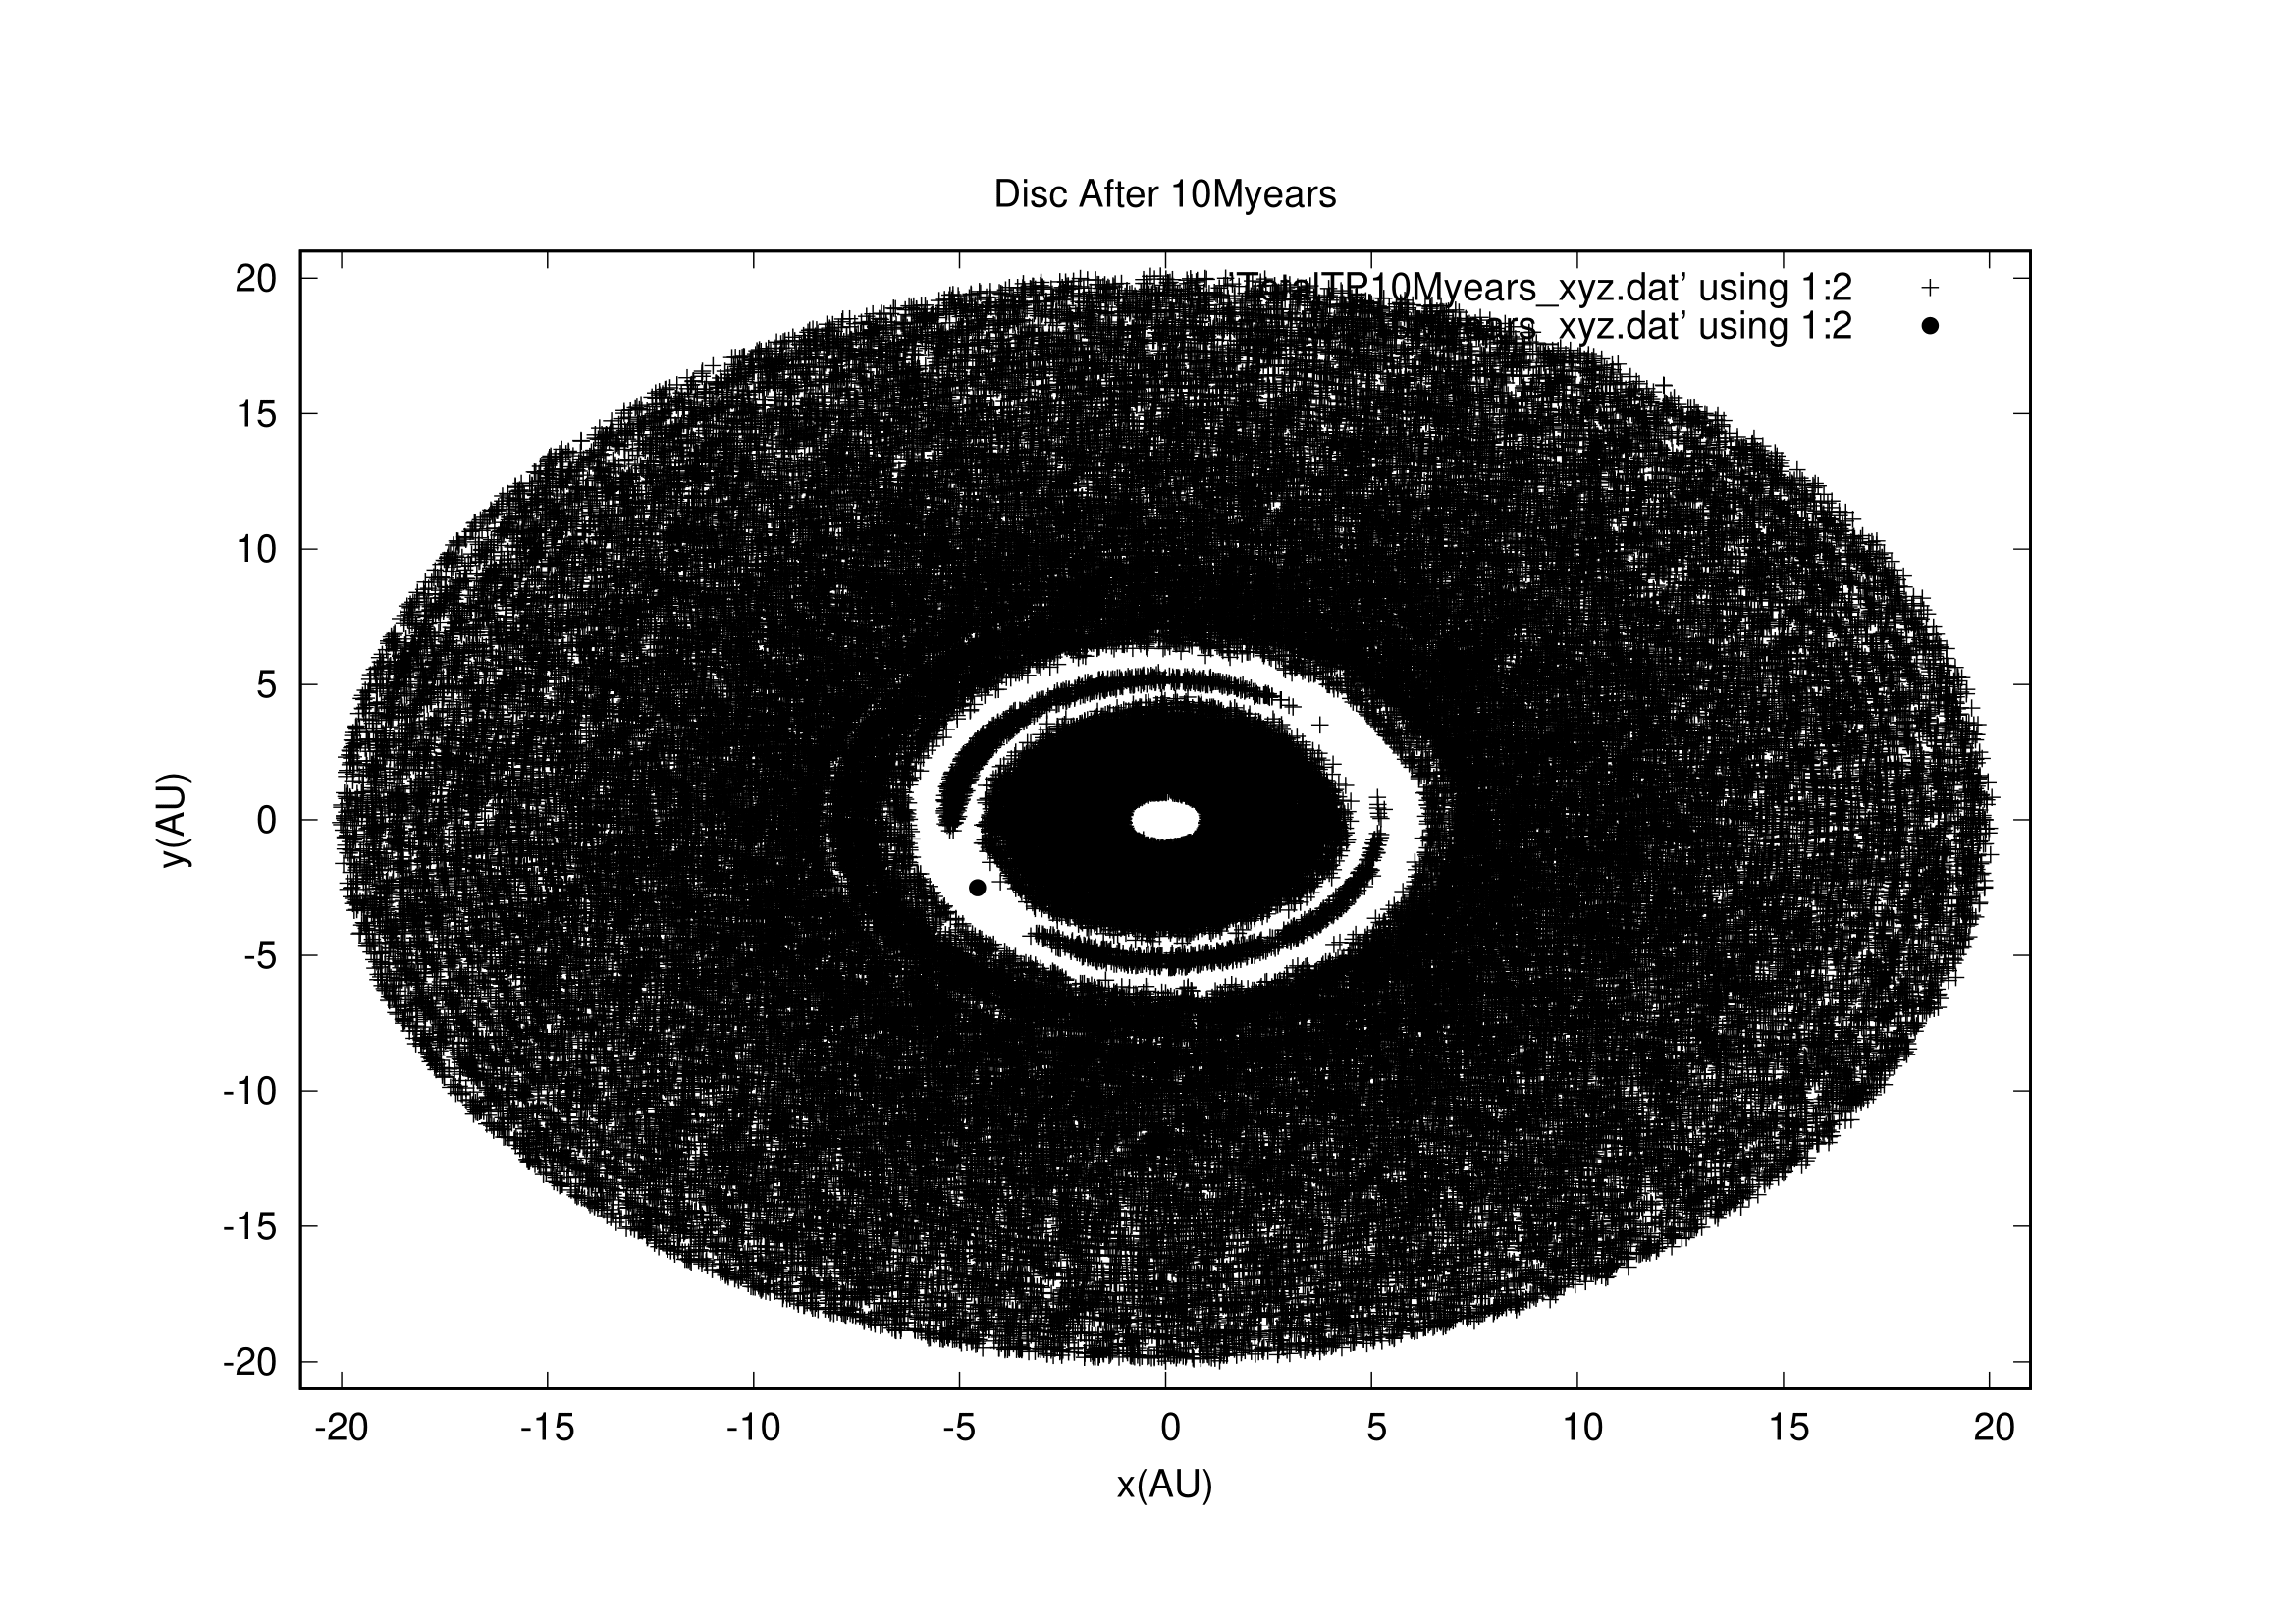
\includegraphics[scale=0.44]{TotalTP10Myears_xyz}
  \caption{Δίσκος τη Χρονική στιγμή $t_1=10 \; Myrs$}\label{fig:DiscAfter10Myear}
\end{figure}

Η θέση κάθε {\en test particle} που παρουσιάζεται στο επίπεδο $x-y$ συμβολίζεται με <<+>> , ενώ η θέση του Δία με <<$\bullet$>> και αυτός ο συμβολισμός θα τηρηθεί σε ολόκληρη την έκταση της εργασίας.\\


Αμέσως μετά την ολοκλήρωση της προσομοιώσης παρατηρούμε ότι:

\begin{itemize}
 \item O αριθμός των {\en test particles} του συστήματος έχει μειωθεί σε σχέση τον αρχικό τους αριθμό.
   \item Έχουν σχηματιστεί δύο ομάδες {\en test particles}, οι οποίες ακολουθούν την τροχιά του πλανήτη και οι θέσεις τους παρουσιάζουν συμμετρία ως προς αυτόν.
    \item Ο πλανήτης έχει <<καθαρίσει>> μεγάλο μέρος της τροχιάς του απο {\en test particles}, δημιουργώντας έναν κενό δακτύλιο στην επιφάνεια του δίσκου και αλλάζοντας έτσι το προφίλ της αριθμητικής του πυκνότητας.
\end{itemize}

\underline{\bf Ανάλυση των Παρατηρήσεων}
\vspace{0.3cm}   
   
Κατα το χρονικό διάστημα της ολοκλήρωσης τα {\en test particles} αλληλεπιδρούν βαρυτικά με τον αστέρα και τον πλανήτη. Αποτέλεσμα αυτής της αλληλεπίδρασης είναι η μεταβολή των στοιχείων της τροχιάς τους σύμφωνα με νόμους της Μηχανικής (όπως αναφέρθηκε ο πλανήτης δεν δέχεται την βαρυτική δύναμη της κατανομής). Έτσι κάποια {\en test particles} άλλοτε αποκτούν τροχιές που τους αναγκάζουν να πέσουνε στην επιφάνεια του αστέρα, άλλοτε ταχύτητες μεγαλύτερες απο την {\it ταχύτητα διαφυγής}\footnote{Ταχύτητα διαφυγής ή παραβολική ταχύτητα ονομάζεται η ελάχιστη ταχύτητα που πρέπει να αποκτήσει, ένα σώμα μάζας $m$ και απόστασης $r$ απο το ελκτικό κέντρο μάζας $Μ$, ώστε να τεθεί σε παραβολική τροχιά και να διαφύγει σε άπειρη απόσταση απο αυτό$\cdot$ $u_\infty = \sqrt{\frac{2G(M+m)}{r}}$} απο τον αστέρα και έτσι διαφεύγουν απο το σύστημα. Τελικά τα {\en test particles} αυτά  χαρακτηρίζονται {\en "not active"}. Ο {\en SWIFT} με τη χρήση του δισδιάστατου πίνακα $istat(NTPMAX,NSTAT)$ ελέγχει μετά απο κάθε {\en timestep} ποιά {\en test particles} είναι {\en "active"} και ποιά {\en "not active"}, καθώς συγκεκριμένοι δείκτες ενημερώνουν το πρόγραμμα σε ποία απο τις δύο καταστάσεις βρίσκεται το κάθε {\en test particle}. Τη χρονική στιγμή {\en $t_1=10 \; Myrs$} τα {\en test particles} που παραμένουν ενεργά στο σύστημα είναι 101294$\cdot$ άρα, απο την \eqref{eq:InitialTPMass}, μάζα του δίσκου είναι:

\begin{equation}\label{eq:t_1TPMass}
 M_{disk} =  101294\times1.746\times10^{24}g = 1.769\times10^{29} g
\end{equation} 
 
Οι δύο ομάδες των {\en test particles} που ακολουθούν την τροχιά του πλανήτη είναι σε συντονισμό $1:1$ με αυτόν και βρίσκονται στα {σημεία ευσταθούς ισορροπίας {\en Lagrange}} $L_4$ και $L_5$ του συστήματος πλανήτη-αστέρα\cite[{\en Chap.~3, Sect.~3.5-.3.7}]{murray1999solar}. Καθώς η τροχιά του πλανήτη είναι σχεδόν κυκλική τα τρίγωνα με κορυφές ΔΗ$L_4$ και ΔΗ$L_5$ είναι ισόπλευρα. Σαν αποτέλεσμα η μια ομάδα βρίσκεται δεσμευμένη σε ένα χώρο 60\degree ,($L_5$), πίσω απο τον πλανήτη (κινούμενη προς αυτόν) και η δεύτερη ομάδα βρίσκεται σε ένα χώρο 60\degree ,($L_4$), μπροστά του (ο πλανήτης κινείται προς αυτήν). Ο συγκεκριμένος συντονισμός είναι ευσταθής για χρόνους συγκρίσιμους με την ηλικία του σύμπαντος, οπότε αν δεν υπάρξει κάποια εξωτερική διαταραχή ο πλανήτης θα εξακολουθήσει να μοιράζεται την τροχιά του με τις δύο αυτές ομάδες διατηρώντας το σύστημα την γεωμετρία του. Οι δύο αυτές ομάδες  μπορούν να ταυτιστούν με τους γνωστούς {\it Τρωικούς} αστεροειδείς του Ηλιακού μας Συστήματος.\\
 
Το εύρος των κενού δακτυλίου {\en (gap)}, που δημιουργήθηκε στον δίσκο, εξαρτάται απο την {\it ακτίνα {\en Hill}} του πλανήτη,\eqref{eq:HillRadius}, άρα κατ' επέκταση απο τον λόγο της μάζας του προς τη μάζα του αστέρα. Ποιοτικά όσο μεγαλύτερη είναι η μάζα του πλανήτη τόσο μεγαλύτερο είναι και το εύρος του δακτυλίου που δημιουργεί στον δίσκο σκόνης. Για τον Δία στο συγκεκριμένο σύστημα μέσω της \eqref{eq:HillRadius} προκύπτει $r_H =0.82615${\en AU}.\\

Όπως αναφέραμε τη χρονική στιγμή {\en $t_0=0 \; sec$} η αριθμητική πυκνότητα των {\en test particles} του δίσκου, είναι σταθερή, οπότε μπορούμε να πούμε ότι η επιφανειακή του πυκνότητα μειώνεται συναρτήσει του τετραγώνου της απόστασης, αφού ο ίδιος αριθμός {\en test particles} διαμοιράζεται σε ολοένα και μεγαλύτερου εμβαδού δακτυλίους. Τη χρονική στιγμή όμως {\en $t_1=10 \; Myrs$} το προφίλ της αριθμητικής πυκνότητας (και κατεπέκταση της επιφανειακής πυκνότητας) του έχουν αλλάξει. Για να μελετήσουμε το νέο αυτό προφίλ αρχικά χωρίσαμε τον δίσκο σε δακτυλίους αριθμού $i$, πάχους $Dr$ και μετρήσαμε τον αριθμό {\en test particles} σε κάθε δακτύλιο συναρτήσει της απόστασης $r$ τους απο το ελκτικό κέντρο. Μέσα απο αυτό το γενικό <<σκανάρισμα>> εξάγαμε το γενικό προφίλ αριθμητικής πυκνότητας του δίσκου. Μετρήσεις έγιναν για τις τιμές:

\begin{table}[h]
 \centering
 \begin{tabular}{l | l | l}
      & $i$ & $Dr${\en (AU)}\\
      \hline \hline
    1 & 204 & 0.1\\
    2 & 120 & 0.17\\
    3 & 85 & 0.24\\          
 \end{tabular}
 \caption{Παράμετροι σκαναρίσματος για την εξαγωγή του γενικού προφίλ αριθμητικής πυκνότητας του δίσκου την {\en $t_1=10 \; Myrs$}}\label{tab:mytable4}
\end{table}

Παρακάτω δίνονται τα διαγράμματα, με τον αριθμό των {\en test particles} $N_{ri}$ συναρτήσει της απόστασης $r$, που προέκυψαν απο τις παραπάνω τιμές για κάθε ζεύγος τιμών:

\newpage

\begin{figure}[h] 
 \begin{subfigure}{0.48\textwidth}
  \includegraphics[width=\linewidth]{GeneralScan0,1}
  \caption{$i=204,Dr=0.1${\en AU}}\label{i204,Dr0.1}
 \end{subfigure}\hspace*{\fill}
 \begin{subfigure}{0.48\textwidth}
  \includegraphics[width=\linewidth]{GeneralScan0,1-Norm}
  \caption{$i=204,Dr=0.1${\en AU-Normalized}}\label{i204,Dr0.1 Norm}
 \end{subfigure}
 \medskip
  
 \begin{subfigure}{0.48\textwidth}
  \includegraphics[width=\linewidth]{GeneralScan0,17}
  \caption{$i=120,Dr=0.17${\en AU}}\label{i120,Dr0.17}
 \end{subfigure}\hspace*{\fill}
 \begin{subfigure}{0.48\textwidth}
  \includegraphics[width=\linewidth]{GeneralScan0,17-Norm}
  \caption{$i=120,Dr=0.17${\en AU-Normalized}}\label{i120,Dr0.17 Norm}
 \end{subfigure}
 \medskip
 
  \begin{subfigure}{0.48\textwidth}
   \includegraphics[width=\linewidth]{GeneralScan0,24}
   \caption{$i=85,Dr=0.24${\en AU}}\label{i85,Dr0.24}
  \end{subfigure}\hspace*{\fill}
  \begin{subfigure}{0.48\textwidth}
   \includegraphics[width=\linewidth]{GeneralScan0,24-Norm}
   \caption{$i=85,Dr=0.24${\en AU-Normalized}}\label{i85,Dr0.24 Norm}
  \end{subfigure}
 \caption{Γενικό Προφίλ Αριθμητικής Πυκνότητας της Κατανομής}
\end{figure}   
 
 Παρατηρώντας τα παραπάνω διαγράμματα μπορούμε να διακρίνουμε τις εξής περιοχές:
\begin{itemize}

 \item Για $0<r \leq 1 \; (AU)$ δεν υπάρχουν {\en test particles} και η αριθμητική πυκνότητα σε αυτή την περιοχή είναι μηδέν. 
 \item Στη συνέχεια για την περιοχή $1 \leq r \leq 3.85 \; (AU)$  ο αριθμος των {\en test particles} παρουσιάζει αύξηση, εκτός απο το σημείο που αντιστοιχεί σε  $r \simeq 3.4 (AU)$. 
 \item Μεταξύ των $3.85 \leq r \leq 7.5 \; (AU)$ εμφανίζεται μια μεγάλη κοίλη, η οποία διαχωρίζεται απο μια κορυφή για $r \simeq 5.2 (AU)$.
 \item O αριθμος των {\en test particles} για $ 7.5 \leq r \leq 20 \; (AU)$ είναι περίπου σταθερός εκτός απο το σημείο που αντιστοιχεί σε  $r \simeq 8.33 (AU)$. Απο εκεί και μετά ο αριθμός των {\en test particles} μειώνεται δραματικά καθώς έχουμε φτάσει στα πέρατα του δίσκου.
  
\end{itemize} 

\underline{\bf Ανάλυση των Διαγραμμάτων}
\vspace{0.3cm} 

Το γεγονός ότι στις περιοχές για $r_1 \simeq 3.4 (AU)$ και $r_2 \simeq 8.33 (AU)$ εμφανίζονται δύο {\it τοπικά ελάχιστα} στον αριθμό των {\en test particles} δεν είναι τυχαίο. Με βάση την \eqref{eq:ResonanceCondition2} παρατηρούμε ότι τα {\en test particles} με ${\en a}_1 \simeq 3.4 (AU)$ βρίσκονται πολύ κοντά στον συντονισμό 2:1 με τον πλανήτη και τα {\en test particles} με ${\en a}_2 \simeq 8.33 (AU)$ στον συντονισμο 1:2 με τον πλανήτη.

\begin{equation}\label{eq:ResonanceCondition3}
 (\frac{\alpha_1}{\alpha_J})^{3/2}=0.53 , \; (\frac{\alpha_J}{\alpha_2})^{3/2}=0.49    
\end{equation}

Οι συντονισμοί αυτοί είναι ασταθείς με αποτελέσμα τα {\en test particles} που βρίσκονται κοντά σε αυτούς να αποκτούν ασταθείς τροχιές σε σχετικά σύντομα χρονικά διαστήματα να μεταβάλλονται τα στοιχεία της τροχιάς τους. Ακόμα βλέπουμε ότι το <<πηγάδι>> στα διαγράμματα για τον συντονισμό τον 1:2, των {\en test particles} με τον πλανήτη, είναι βαθύτερο απο το πηγάδι για τον συντονισμό 2:1 με τον πλανήτη. Η συμπεριφορά αυτή ερμηνεύεται απο την \eqref{eq:ResonanceCondition3}, η οποία μας δείχνει ότι ο πρώτος είναι πιο κοντά στην ακριβή τιμή του συντονισμού, ($0.5$), άρα είναι και πιο ισχυρός.\\

Ουσιαστικά παρατηρώντας την γεωμετρία του δίσκου, Σχήμα:~\ref{fig:DiscAfter10Myear}, σε συνδυασμό με τα παραπάνω διαγράμματα αριθμητικής κατανομής των {\en test particles}, μπορούμε να κατανοήσουμε ότι η ενδιάμεση κορυφή αντιστοιχεί στις ομάδες {\en test particles} που εντοπίζονται στα {σημεία ευσταθούς ισορροπίας {\en Lagrange}} ($L_4$, $L_5$) και χρήζει πιο λεπτομερή ανάλυση.\\

Ας υποθέσουμε ότι κινούμαστε ακτινικά απο το κέντρο του δίσκου προς την άκρη του σε μια τυχαία διεύθυνση (τυχαία αζιμουθιακή γωνία θ)\footnote{Η γνωστή αζιμουθιακή γωνία των πολικών συντεταγμένων} έως ότου συναντήσουμε τα {\en test particles} των περιοχών $L_4$ και $L_5$ . Ακολουθώντας τον παραπάνω συλλογισμό είναι εμφανές ότι καθώς κινηθούμε ακτινικά το {\bf αν} θα τα συναντήσουμε {\it εξαρτάται απο την γωνία θ} στην οποία θα επιλέξουμε να κινηθούμε$\cdot$ καθώς η δακτυλοειδής αυτή περιοχή, σε αντίθεση με τις άλλες δύο, δεν είναι συνεχής αλλά διαχωρίζεται στη διάμετρο που ταυτίζεται με την διεύθυνση εντοπισμού του πλανήτη. Η ύπαρξη της ενδιάμεσης αυτής κορυφής, σε συνδυασμό με τον κενό δακτύλιο, θα μας απασχολίσει ιδιαίτερα καθώς αποτελούν την \underline{\bf{ ένδειξη ύπαρξης πλανήτη}} στον δίσκο. Τέλος τα δύο <<πηγάδια>> δεξιά και αριστερά της ενδιάμεσης κορυφής αντιστοιχούν στον κενό δακτύλιο που δημιουργεί ο πλανήτης στην τροχία του. Ο δακτύλιος αυτός, προφανώς δεν είναι απόλυτα κενός, αλλα περιέχει τα {\en test particles} των περιοχών $L_4$, $L_5$ για αυτό και εμφανίζεται η κορυφή όπως αναφέρθηκε.\\

Το γεγονός ότι για αποστάσεις $r > 8.33 (AU)$ η αριθμητική πυκνότητα των {\en test particles} είναι σχεδόν σταθερή μας σηματοδοτεί και το όριο της κυριαρχίας του βαρυτικού δυναμικού του Δία. Φυσικά η βαρυτική του δύναμη εξακολουθεί να ασκείται στα {\en test particles} όμως δεν είναι ικανή να μεταβάλλει έντονα τα στοιχεία της τροχιάς τους$\cdot$ εκτός για κάποια απο αυτά που ίσως βρεθούν σε κάποιο συντονισμό ασταθούς ισορροπίας με τον Δία.\\

Στο σημείο αυτό προκειμένου να μελετήσουμε σε μεγαλύτερο βάθος την γεωμετρία που απέκτησε ο δίσκος λόγω της παρουσίας του πλανήτη, αλλα και τις χαρακτηριστικές περιοχές της κατανομής, συντάχθηκε ένα {\en script} με την ονομασία {\en {\it ScanDiskFixed.f}}. Σύμφωνα με αυτό χωρίσαμε επιπλέον τον δίσκο, με αρχή την διεύθυνση του πλανήτη την {\en $t_1=10 \; Myrs$} , σε ${\en j=36}$ διαμετρικές διευθύνσεις ανα 10\degree \; και επαναλάβαμε την διαδικασία <<σκαναρίσματος>> του δίσκου δοκιμάζοντας διαφορετικές τιμές παραμέτρων. Έστω πχ η διεύθυνση αναφοράς είναι η θ$=0\degree$ και θ$=180\degree$, η επόμενη είναι η θ$=10\degree$ και θ$=190\degree$ κ.ο.κ.\\
Τώρα μετρήθηκε ο αριθμός {\en test particles} σε κάθε διεύθυνση με εύρος $\pm$ $Dth\degree$, σε κάθε έναν δακτυλίο πάχους $Dr$ απο τους $i$ δακτυλίους. Ισοδύναμα  μετρήθηκε ο αριθμός των {\en test particles} σε κάθε <<κελί>> $[i,j]$, όπου $i=1,2,3,..$ και $j=1,2,3,...,36$. Μετρήσεις έγιναν για τις τιμές:

\begin{table}[h]
 \begin{subtable}[h]{0.3\textwidth}
   \centering
   \begin{tabular}{l | l | l}
      & $i$ & $Dr${\en (AU)}\\
    \hline \hline
    1 & 204 & 0.1\\
    2 & 120 & 0.17\\
    3 & 85 & 0.24\\
    \end{tabular}
    \caption{$Dth=\pm$ $10\degree$}\label{tab:+-10degree}
 \end{subtable}
 \hfill      
 \begin{subtable}[h]{0.3\textwidth}
   \centering
   \begin{tabular}{l | l | l}
      & $i$ & $Dr${\en (AU)}\\
    \hline \hline
    1 & 204 & 0.1\\
    2 & 120 & 0.17\\
    3 & 85 & 0.24\\
    \end{tabular}
    \caption{$Dth=\pm$ $15\degree$}\label{tab:+-15degree}  
  \end{subtable}
  \hfill  
 \begin{subtable}[h]{0.3\textwidth}
   \centering
   \begin{tabular}{l | l | l}
      & $i$ & $Dr${\en (AU)}\\
    \hline \hline
    1 & 204 & 0.1\\
    2 & 120 & 0.17\\
    3 & 85 & 0.24\\
    \end{tabular}
    \caption{$Dth=\pm$ $20\degree$}\label{tab:+-20degree}   
 \end{subtable}
\caption{Τιμές των Διαφόρων Παραμέτρων <<Σκαναρίσματος>> του Δίσκου}\label{tab:Scans}
\end{table}

Είναι φανερό ότι οι 36 διευθύνσεις ανα $10\degree$ έχουν σαν αποτέλεσμα να μετρηθεί δύο φορές ο αριθμός των {\en test particles} του δίσκου. Επιπλέον το εύρος $\pm$ $Dth\degree$ σε κάθε διεύθυνση έχει σαν αποτέλεσμα επικαλύψεις μεταξύ των περιοχών μέτρησης {\en test particles}. Για τους παραπάνω λόγους ο αριθμός των {\en test particles} κανονονικοποιήθηκε σύμφωνα με το εμβαδόν επικάλυψης για τα διαφορετικά εύρη <<σκαναρίσματος>>. Επίσης κρατήσαμε τις μετρήσεις των 18 πρώτων διαμετρικών διευθύνσεων, ($j=1,2,3,...,18$), καθώς αύτες περιλαμβάνουν μια πλήρη μέτρηση των {\en test particles} του δίσκου ($18\times10\degree=180\degree$) και οι επόμενες 18 είναι αντίστοιχες καθώς μετριούνται τα {\en test particles} του δίσκου για δεύτερη φορά.

Καταλήξαμε να κρατήσουμε τις τιμές των παραμέτρων που δίνουν τον διαχωρισμό του δίσκου σε $i=120$ δακτυλίους πάχους $Dr=0.17${\en AU}, δηλαδή 

\begin{table}[h]
 \centering
 \begin{tabular}{l | l | l}
     $\pm$ $Dth\degree$ & $i$ & $Dr${\en (AU)}\\
      \hline \hline
    $\pm$ 10 & 120 & 0.17\\
    $\pm$ 15 & 120 & 0.17\\
    $\pm$ 20 & 120 & 0.17\\      
 \end{tabular}
 \caption{Παράμετροι Διαχωρισμού του Δίσκου- <<Σκαναρισματος>>}\label{tab:ScanParameters}
\end{table}

 Τελικά πήραμε 54 διαφορετικές μετρήσεις του αριθμού των {\en test particles} για κάθε <<κελί>> ενός δακτυλίου $Dr_i$, όπου $i=1,2,...,120$. Στη συνέχεια βρήκαμε τον {\it μέσο όρο του αριθμού των {\en test particles}}, $Mean N_{ri}$, για κάθε <<κελί>> δακτυλίου $i$ και πάχους $Dr_i$ καθώς και το <<κελί>> με τον μέγιστο αριθμό {\en test particles}, $N_{max}$, και αυτό με τον ελάχιστο αριθμό {\en test particles}, $N_{min}$. Παρακάτω δίνεται η γραφική παράσταση μαζί με την {\it τυπική απόκλιση} των μετρήσεων στον μέσο όρο:
 \newpage

\begin{figure}[h]
  \centering
  \includegraphics[scale=0.5]{MeanNumDensity}
  \caption{Μέσος Όρος του Αριθμού των {\en Test Particles} σε κάθε Δακτύλιο $Dr_i$\\
  Με κόκκινο χρώμα δίνεται η $N_{max}(r)$, με πράσινο η $N_{min}$ και ο $Mean N$ μπλέ}\label{fig:MeanNb}
\end{figure}  

Βλέπουμε ότι σε κάθε δακτύλιο $r_i$, \underline{με εξαίρεση την περιοχή του πλανήτη}, οι τιμές της {\it τυπικής απόκλισης} δεν είναι μεγάλες, αυτό σημαίνει ότι η διαφορά του αριθμού των {\en test particles} μεταξύ των <<κελιών>> με το ίδιο $r$ αλλά διαφορετική διεύθυνση θ (πχ τα <<κελιά>> [3,1],[3,2],[3,3] κ.ο.κ.) δεν είναι μεγάλη ή ισοδύναμα έχουμε περίπου ομοιόμορφα κατανεμημένα τα {\en test particles} του κάθε δακτυλίου σε αυτόν και ο συνολικός τους αριθμός μπορει να προσεγγιστεί αρκετά ικανοποιητικά απο τον μέσο όρο $MeanN_{ri}\forall i=1,2,...,120$. Αντίθετα ο αριθμός των {\en test particles}, για $r$ κοντά στην $r_J = 5.2044${\en AU}, παρουσιάζει μεγάλη διασπορά τιμών$\cdot$ σε κάποια διεύθυνση ο αριθμός των {\en test particles} αγγίζει το μηδέν ενώ ταυτόχρονα ο αριθμός {\en test particles} σε άλλη διεύθυνση παρουσιάζει μεγάλες τιμές. Αυτή ακριβώς η μη ισοτροπική κατανομή των {\en test particles} στη συγκεκριμένη απόσταση $r$ αποτελεί ένδειξη ότι υπάρχει ένα μαζικό σώμα σε αυτήν περίπου την απόσταση. Η παρουσία του σώματος και κατ' επέκταση η βαρυτική του επιρροή προκαλεί την μεγάλη διασπορά στον αριθμό των {\en test particles}, η οποία αντίστροφα είναι η δυναμική <<υπογραφή>> της παρουσίας του.\\

\newpage

Με δεδομένο το προφίλ αριθμητικής πυκνότητας του δίσκου μπορούμε να εξάγουμε και το προφίλ της επιφανειακής του πυκνότητας, αφού γνωρίζουμε εμβαδόν κάθε δακτυλίου και την μάζα του καθε {\en test particle}. Παρακάτω δίνεται το διάγραμμα επιφανειακής πυκνότητας του δίσκου:


\begin{figure}[h]
  \centering
  \includegraphics[scale=0.5]{SurfDens(units)}
  \caption{Επιφανειακή Πυκνότητα σε κάθε Δακτύλιο $Dr_i$ Συναρτήσει της Απόστασης\\
  Με κόκκινο χρώμα δίνεται η $\Sigma_{max}(r)$, με πράσινο η $\Sigma_{min}(r)$ και ο $\Sigma(r)$ μπλέ}\label{fig:SurfDens}
\end{figure}

Φαίνεται καθαρά η {\it εκθετική μείωση} της επιφανειακής πυκνότητας συναρτήσει της απόστασης μέχρι το όριο όπου το βαρυτικό δυναμικό του πλανήτη παύει να παίζει τον κυρίαρχο ρόλο. Απο εκεί και μετά η καμπύλη της επιφανειακής πυκνότητας είναι πιο ομαλή και συνεχίζει να μειώνεται συναρτήσει της απόστασης με μικρότερο όμως ρυθμό. Επίσης φαίνονται καθαρά τα δύο τοπικά ελάχιστα που αντιστοιχούν στους μεγάλους ημιάξονες $\alpha_1 \simeq 3.4 (AU)$ και $\alpha_2 \simeq 8.33 (AU)\cdot$ καθώς τα {\en test particles} βρίσκονται πολύ κοντά στους συντονισμούς 2:1 και 1:2 με τον πλανήτη.\\

Στο σημείο αυτό αξίζει να σημειωθεί ότι το 55.25\% της συνολικής μάζας του δίσκου βρίσκεται μεταξύ $1$ με $~5 AU$, δηλαδή σε έναν δακτύλιο εύρους $~4AU$. Το υπόλοιπο 44.75\% κατανέμεται απο $~5$ εώς $20.4 AU$, δηλαδή σε ένα δακτύλιο εύρους $~15AU$. Αυτή η μεγάλη διαφοροποίηση στην επιφανειακή πυκνότητα του δίσκου θα είναι πολύ σημαντική για τα αποτελέσματα του μοντέλου μας όπως θα δούμε παρακάτω.\\

Τέλος για να προσδιορίσουμε την αντίστοιχη καμπύλη, \ref{eq:SurfaceProfile}, που περιγράφει το προφίλ επιφανειακής πυκνότητας του δίσκου βάση των δεδομένων μας αποβάλλαμε τους δακτυλίους απόστασης $<1 AU$, καθώς δεν εμπεριέχουν καθόλου ύλη. Παρακάτω δίνεται το διάγραμμα επιφανειακής πυκνότητας του δίσκου για $r \geq1 AU$:

\begin{figure}[h]
  \centering
  \includegraphics[scale=0.5]{SurfDens(units)2}
  \caption{Επιφανεικαή Πυκνότητα σε κάθε Δακτύλιο $Dr_i$, όπου $r \geq1 AU$ Συναρτήσει της Απόστασης\\
  Με κόκκινο χρώμα δίνεται η $\Sigma_{max}(r)$, με πράσινο η $\Sigma_{min}(r)$ και ο $\Sigma(r)$ μπλέ}\label{fig:SurfDens2}
\end{figure}

όπου τελικά $\Sigma(r) = 8.53889\times r^{-1.20529} \frac{g}{cm^2}$.


